\documentclass[12pt]{article}
\usepackage{graphicx}
\begin{document}
\title{Computer Science M151B, Homework 5}
\date{May 7th, 2018}
\author{Michael Wu\\UID: 404751542}
\maketitle

\section*{Problem 1}

Yes, the \texttt{PCSrc} signal could be computed in the \texttt{EX} stage, as the zero of the ALU output and the \texttt{Branch} signal are both
available in \texttt{EX}. An advantage of making this change would be to reduce the branch penalty from three cycles to two cycles, since we can
update the program counter one cycle earlier. However, since this adds an \texttt{and} gate to the output of the ALU, this could potentially
lead to a higher cycle time. The book shows a better implementation where the branch computed in the \texttt{ID} stage, reducing the branch penalty
to one cycle, which is why this change is not used.

\section*{Problem 2}

\paragraph{a)}

The value of \texttt{PCSrc} is 0 when this instruction is in the \texttt{MEM} stage. This is because there is no branching going on, so the program counter
should update normally.

\paragraph{b)}

The value of \texttt{PCSrc} is 1 when this instruction is in the \texttt{MEM} stage. This is because this branch instruction checks if register \texttt{\$5}
is equal to itself, which must be true. So the branch will be taken and the program counter will be updated to the address given in the branch instruction.

\section*{Problem 3}

This series of instructions will execute over 9 cycles. On the fifth cycle, the first \texttt{add} instruction is in the \texttt{WB} stage, so register \texttt{\$2} is
written. Additionally, the third \texttt{add} instruction is in the \texttt{ID} stage, so the registers \texttt{\$6} and \texttt{\$1} are being read.

\section*{Problem 4}

\begin{figure}[!ht]
        \hspace*{-4cm}
        \begin{center}
                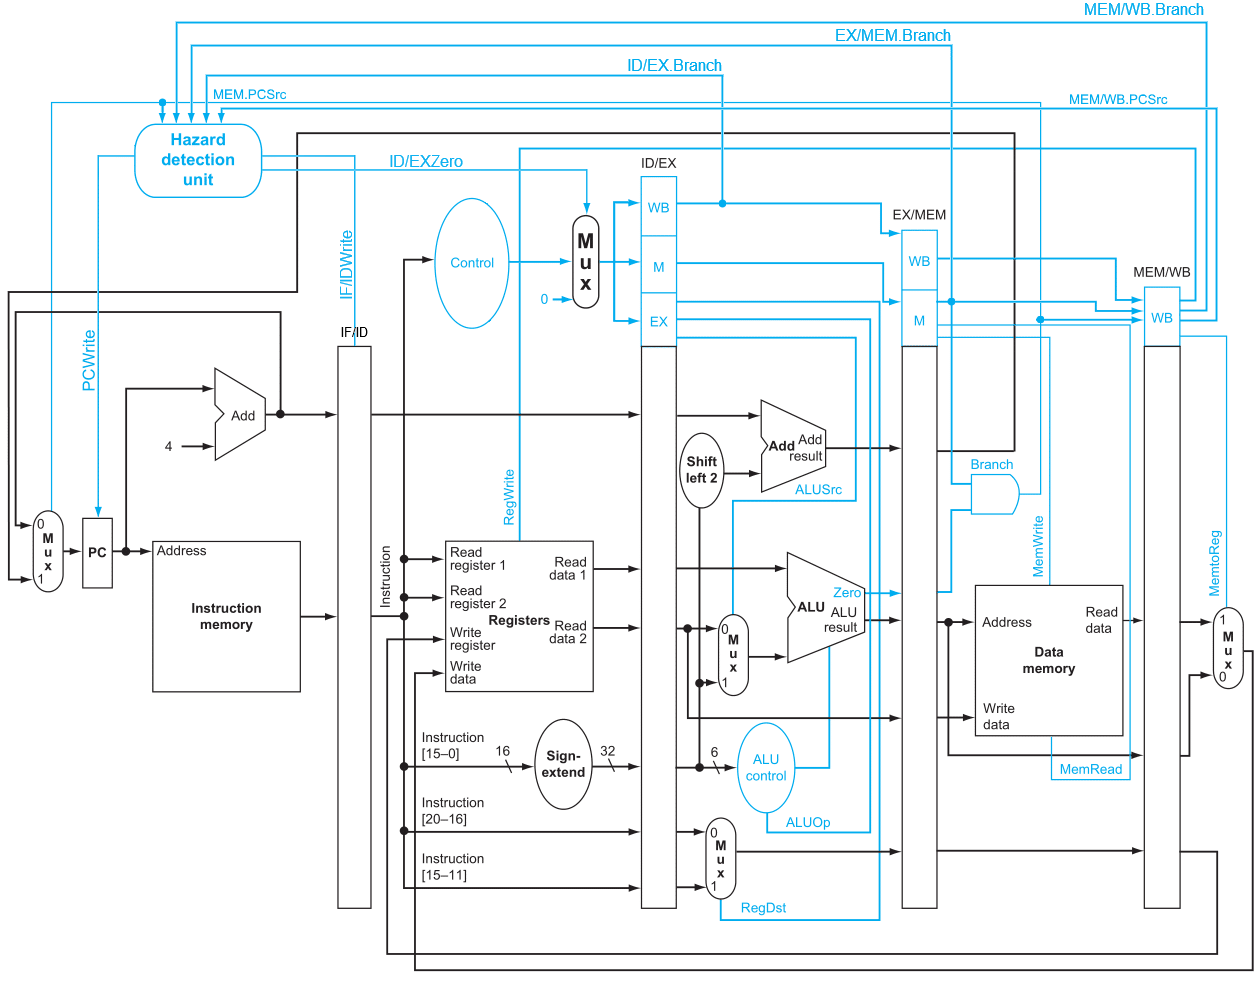
\includegraphics[width=5in]{problem4.png}
        \end{center}
        \hspace*{-4cm}
\end{figure}

The modified hazard detection unit is shown above. The goal of this modification is to always stall for three cycles after every branch.
I have added the \texttt{Branch} control signal to the \texttt{MEM/WB} registers, so that a signal is available to determine if a branch instruction
is in the \texttt{WB} stage. I have also added the \texttt{MEM/WB.PCSrc} signal to aid in fetching a new instruction if the branch is taken. The hazard detection
unit stalls by injecting 0 into the \texttt{ID/EX} registers. It also sets \texttt{IF/IDWrite} and \texttt{PCWrite} to 0 to prevent a new instruction
from being loaded.

The logic for the outputs of the hazard detection unit is shown below.
\begin{verbatim}
if (ID/EX.Branch or EX/MEM.Branch or MEM/WB.Branch)
  then ID/EXZero = 1 else ID/EXZero = 0

if (MEM/WB.PCSrc != 1 and
  (ID/EX.Branch or EX/MEM.Branch or MEM/WB.Branch))
    then IF/IDWrite = 0 else IF/IDWrite = 1

if (MEM.PCSrc != 1 and MEM/WB.PCSrc != 1 and
  (ID/EX.Branch or EX/MEM.Branch or MEM/WB.Branch))
    then PCWrite = 0 else PCWrite = 1
\end{verbatim}
Note that I set \texttt{PCWrite = 1} when \texttt{MEM.PCSrc = 1} to allow for the branch to update the program counter if it is taken. I then
set \texttt{PCWrite = 1} and \texttt{IF/IDWrite = 1} when \texttt{MEM/WB.PCSrc = 1} to allow for the instruction at the branch target address to be read, and the
program counter to be updated in the next cycle.

\pagebreak

\section*{Problem 5}

\begin{figure}[!ht]
        \hspace*{-4cm}
        \begin{center}
                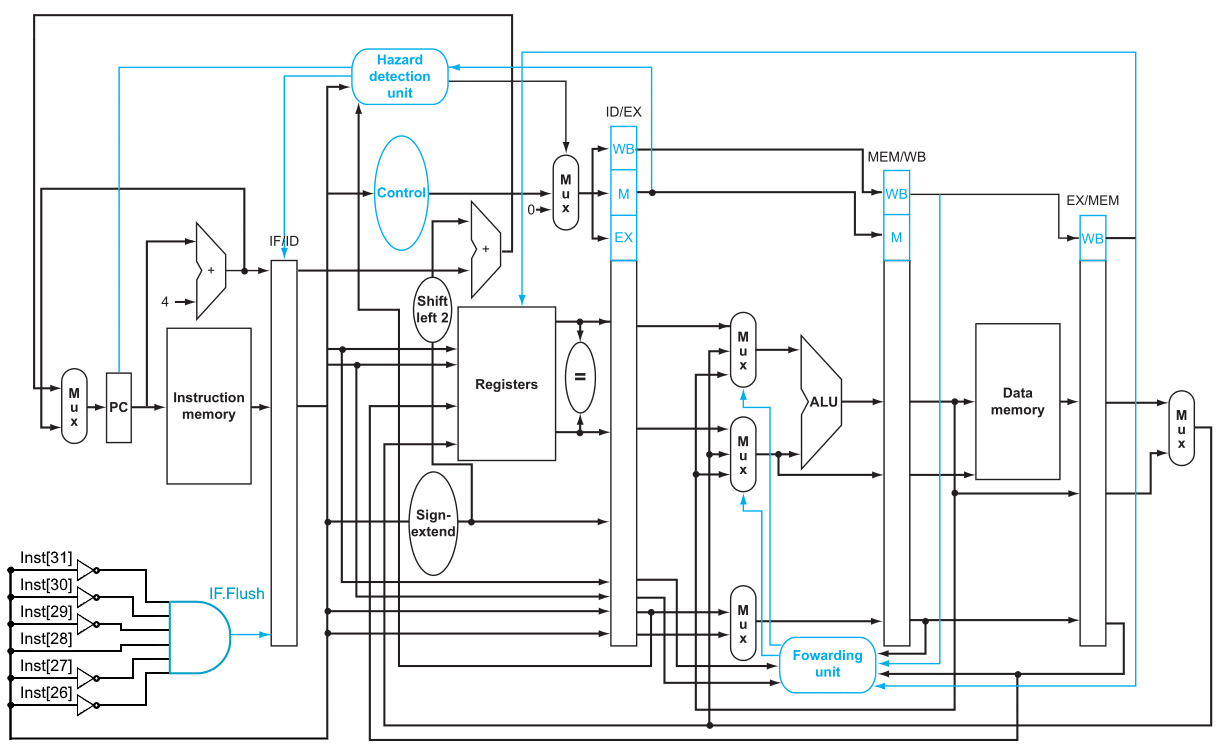
\includegraphics[width=4.8in]{problem5a.png}
        \end{center}
        \hspace*{-4cm}
\end{figure}

\paragraph{a)}

Since the \texttt{IF.Flush} signal is asserted whenever a branch intstruction occurs, this corresponds to asserting it when an opcode of 4 is read. So this
circuit implements that logic.

\begin{figure}[!ht]
        \begin{center}
                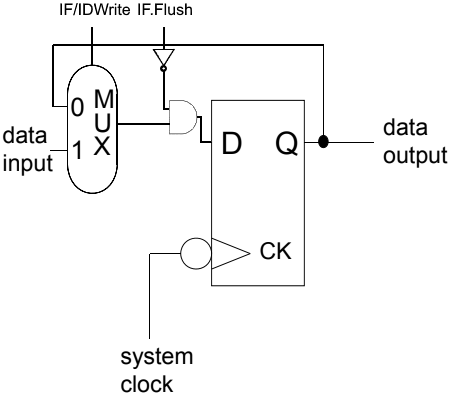
\includegraphics[width=2.5in]{problem5b.png}
        \end{center}
\end{figure}

\paragraph{b)}

The \texttt{IF.Flush} signal will be used to clear out the register by using a gate as shown in the figure above. The gate is placed after the
multiplexer controlled by \texttt{IF/IDWrite}, so that \texttt{IF.Flush} has precendence over \texttt{IF/IDWrite}.

\section*{Problem 6}

The updated code will be
\begin{verbatim}
addi $r6,  $r6,  12
sw   $r16, $r6
addi $r6,  $r6,  -4
lw   $r16, $r6
beq  $r5,  $r4,  Label
add  $r5,  $r1,  $r4
slt  $r5,  $r15, $r4
\end{verbatim}
which increases the number of instructions to 7. Since the length of the pipeline decreases by one cycle, this will require 10 cycles to execute.
Previously with the 5 stage pipeline, there were 5 instructions which required 9 cycles to execute. So our speedup is
\[\frac{9}{10}=0.9\]
which indicates that we actually get worse performance by making this change.

\section*{Problem 7}

With stall-on-branch and the branch outcome being determined in the \texttt{EX} stage, the code will take 11 cycles to execute. Determining the branch
outcome in the \texttt{ID} stage reduced the branch penalty by one, which makes the code take 10 cycles to execute. Since we assume that the latencies
of each stage are as shown in the given table, our clock cycles will be the same for either implementation. Thus determining the branch outcome in the \texttt{ID}
stage gives a speedup of
\[\frac{11}{10}=1.1\]
relative to determining the branch outcome in the \texttt{EX} stage.

\section*{Problem 8}

The opcode must contain at least 8 bits, and each register field must contain at least 6 bits. So that leaves at most 12 bits for the immediate field.
Thus the maximum range of the immediate value is from \(-2048\) to \(2047\) in decimal.

\section*{Problem 9}

Implementing this code in MIPS using indexed addressing would yield the following code.
\begin{verbatim}
add  $t0, $zero, $zero
addi $t1, $zero, 10
sll  $t2, $t0,   2
add  $t2, $t2,   $a1
sll  $t3, $t0,   3
add  $t3, $t3,   $a0
lw   $t4, 0($t2)
add  $t4, $t4,   $t0
sw   $t4, 0($t3)
addi $t0, $t0,   1
bne  $t0, $t1,   -9
\end{verbatim}
Implementing this code in PowerPC using update addressing would yield the following code.
\begin{verbatim}
      xor   r1, r1, r1
      addi  a1, a1, -4
      addi  a0, a0, -8
loop: lwzu  r2, 4(a1)
      add   r2, r2, r1
      stwu  r2, 8(a0)
      addi  r1, r1, 1
      cmpwi r1, 10
      bne   loop
\end{verbatim}

\end{document}